\documentclass{article}
\usepackage{graphicx}
\usepackage{hyperref}
\usepackage{tcolorbox}
\usepackage{parskip}
\usepackage{enumitem}
\usepackage[authoryear]{natbib}
\usepackage{mdframed}
\usepackage[margin=1in]{geometry}
\usepackage{booktabs}
\usepackage{amsmath}

\title{\textbf{Simon Opsahl}\\AI, Decision Making, and Society\\6.3950/6.3952, Fall 2024\\Pset 5 -- Online Platforms}

\begin{document}
\date{Due: October 23, 2024 (by 11:59 PM)}

\maketitle
\section*{}

AI plays a central role in shaping online platforms, influencing both \textit{what we say} and \textit{what we see}. In this problem set, you will explore how AI algorithms mediate our interactions and determine what content we consume across online platforms. This problem set has 4 parts:
\begin{itemize}
    \item Problem 1: Recommender Systems
    \item Problem 2: Content Moderation
    \item Problem 3: User Engagement
    \item Problem 4: Misinformation
\end{itemize}


Please submit your assignment as a PDF compiled from this LaTeX template.

\newpage

\section*{Problem 1: Recommender Systems}
\textit{Note: This problem will directly build on the activity in Recitation 5 on 10/11. You may want to wait until after recitation to begin this problem.}

\bigskip 
\textbf{Optional Background Reading:}
\begin{itemize}
\item \href{https://www.nvidia.com/en-us/glossary/recommendation-system}{Overview of recommendation systems and different architectures} (NVIDIA)
\item \href{https://www.mdpi.com/2079-9292/11/1/141}{A Survey of Recommendation Systems: Recommendation Models, Techniques, and Application Fields} (Ko et al. 2022)
\item \href{https://dl.acm.org/doi/pdf/10.1145/3632297}{Building Human Values into Recommender Systems: An Interdisciplinary Synthesis and Open Problems} (Stray et al. 2023)
\end{itemize}
\bigskip 

Recommender systems are algorithms designed to recommend relevant items to users based on their preferences, behaviors, or characteristics. They enable personalized experiences across various online platforms, including e-commerce, streaming services, and social media. By leveraging historical data collected on users, these systems can identify patterns and predict user preferences, with the goal of improving user engagement and satisfaction. 

This problem will build on the activity in Recitation 5 where we explored building a recommender system using the MovieLens dataset. To complete this exercise, you will need to make a copy of this \href{https://colab.research.google.com/drive/1cePNNiv2fVCfrrQGHov4kUJZDmViH5M8?usp=sharing}{Colab notebook} and fill in some sections. However, you will provide all your answers in this LaTeX document. 


\subsection*{Exploratory Data Analysis}

First, you will perform some exploratory data analysis about the highest rated movies. Run the cells in the notebook until \textit{Part 1: Exploratory Data Analysis}. Then, fill in your code for that section, and answer the questions below.

\textit{Note: The Gemini auto-complete feature may be helpful for filling out the code in this section. If you type pseudo-code as comments in the cell, you should see that Gemini will suggest code for you. This \href{https://pandas.pydata.org/docs/user_guide/10min.html}{overview of the Pandas python library} may also be helpful.} 

\textbf{1. Fill in your code for ``Part 1: Exploratory Data Analysis'' to answer the following questions.}
\begin{enumerate}[label=\Alph*.]
\item What movies have an average rating of 4.5 or higher and were released in 2000 or later?
\item What are the top 5 movies with the highest accumulated rating? Accumulated rating is the sum of ratings over all users.
\end{enumerate}

\bigskip

\begin{mdframed}
\begin{enumerate}[label=\Alph*.]
\item There are only two movies in the dataset that fit this criteria: Bittersweet Motel and Skipped Parts.
\item When ordered by accumulated rating, the top 5 movies in order were American Beauty, Star Wars IV, Star Wars V, Star Wars VI, and Saving Private Ryan.
\end{enumerate}
\end{mdframed}

\bigskip


\textbf{2. Using the plot that compares average rating and accumulated rating, answer the following.}
\begin{enumerate}[label=\Alph*.]
\item What is the shape of the distribution for average rating?
\item What is the shape of the distribution for accumulated rating?
\item What is the general relationship between the accumulated rating and average rating?
\item What is the relationship between the accumulated rating and average rating for movies with a very high or very low average rating? 
\item Based on the MovieLens data, suppose we want to recommend 5 movies to someone who has not rated any movies. Should we select the 5 movies based on the highest average rating or the highest accumulated rating?
\end{enumerate}


\bigskip

\begin{mdframed}
\begin{enumerate}[label=\Alph*.]
\item The shape of the average rating is bimodal, with one mode around 3.5 and another around 1 star.
\item Accumulated rating is right skewed, with most of the accumulations less than 10.
\item The accumulated rating and average rating tend to have a positive correlation. 
\item Movies with very low average rating have very low accumulated rating. Movies with high average rating are not as clear, however, though there is an increase in accumulated rating.
\item I would recommend the 5 movies that maximize the product of highest accumulated score to average ratio, or the ones that were reviewed frequently AND had a high average score. This corresponds to the movies in the top right corner of the plot.
\end{enumerate}
\end{mdframed}

\bigskip

\subsection*{Understanding the Recommendations Model}

For this part of the problem (Questions 3-6), you will not need the notebook. 

As we discussed in Recitation, the notebook builds a recommendation model that is based on the $K$-Nearest Neighbors ($K$-NN) algorithm. Specifically, we generate recommendations for a given user using the following procedure:
\begin{enumerate}
    \item \textit{Identify the $K$ nearest neighbors}: Find the $K$ users that are most similar to the current user based on their movie ratings. 
    \item \textit{Generate a candidate set of possible recommendations}: Find the set of $T$ movies that have the highest (accumulated) rating based on the ratings of the $K$ nearest neighbors, excluding movies that the user has already watched/rated. 
    \item \textit{Recommend 5 movies using a weighted lottery}: Choose 5 movies from the candidate set of $T$ movies using a weighted lottery, where the probability of selecting each movie is based on its accumulated rating from the K nearest neighbors.
\end{enumerate}

\subsubsection*{Similarity Metric}

In our implementation, we use \href{https://en.wikipedia.org/wiki/Cosine_similarity}{Cosine similarity} because the vectors are sparse (i.e. there are many movies, but each person has only rated a few). The formula for cosine similarity between two vectors \( \mathbf{A} \) and \( \mathbf{B} \) is:

\[
\text{cosine\_similarity}(\mathbf{A}, \mathbf{B}) = \frac{\mathbf{A} \cdot \mathbf{B}}{\|\mathbf{A}\| \|\mathbf{B}\|}   = \frac{\sum_{i=1}^{n} A_i B_i}{\sqrt{\sum_{i=1}^{n} A_i^2} \sqrt{\sum_{i=1}^{n} B_i^2}}
\]



\begin{table}[h]
    \centering
    \caption{Historical Movie Ratings for Question 4}
    \begin{tabular}{llllll}
        \toprule
        \textbf{User} & \textbf{Movie 1} & \textbf{Movie 2} & \textbf{Movie 3} & \textbf{Movie 4} & \textbf{Movie 5} \\
        \midrule
        Aleksander & - & 2 & - & 3 & - \\
        Ashia & 4 & - & 1 & - & 4 \\
        Manish & 2 & 4 & - & - & 5 \\ 
        \midrule 
        Dylan & 5 & 1 & 2 & - & - \\
        \bottomrule
    \end{tabular}
    \label{tab:movie_ratings}
\end{table}


\textbf{3. Answer the following questions about Cosine similarity based on Table 1.}
\begin{enumerate}[label=\Alph*.]
\item Given that we are using Cosine similarity, what value should we use to fill in missing ratings? Briefly justify your answer in a few sentences.
\item Who has the highest Cosine similarity to Dylan? Rank the other users (Aleksander, Ashia, Manish) in terms of their similarity to Dylan, from highest to lowest.
\end{enumerate}
\bigskip
\begin{mdframed}
\begin{enumerate}[label=\Alph*.]
\item When we have missing ratings, we should use a null value. For all intents and purposes, this corresponds to a zero to demonstrate no contribution to the sum. 
\item The user cosine similarities are explored below:
    \begin{itemize}
        \item Aleksander: $\frac{2*1}{\sqrt{2^2 + 3^2}\sqrt{5^2+1^2+2^2}} = \frac{2}{\sqrt{390}}=0.101$
        \item Ashia: $\frac{4*5 + 1*2}{\sqrt{4^2 + 1^2 + 4^2}\sqrt{5^2+1^2+2^2}} = \frac{22}{\sqrt{990}}=0.699$
        \item Manish: $\frac{2*5 + 4*1}{\sqrt{2^2 + 4^2 + 5^2}\sqrt{5^2+1^2+2^2}} = \frac{14}{\sqrt{1350}}=0.381$
    \end{itemize}
    Ashia has the highest cosine similarity with Dylan, followed by Manish, then Aleksander.
\end{enumerate}
\end{mdframed}
\bigskip

\subsubsection*{Utility Based on Expected Ratings}

Recall from Recitation how analyzed the ``utility'' of recommendations.  If a platform were to use our recommendation model, they might define utility based on user satisfaction. One way to measure this utility is by looking at the ratings users give to the movies they are recommended.

However, we can't directly observe user ratings without deploying the model. Instead, we can calculate an estimate of \textit{expected utility}. To do this, we consider the genre of each recommended movie and the average rating that the user has historically given to that genre.

For example, if Dylan has rated comedy movies with an average of 4 stars, then the expected utility of recommending a comedy movie to him would be 4 stars. This approach allows us to estimate how satisfied Dylan might be with a comedy recommendation based on his past ratings.





\begin{table}[h]
    \centering
    \caption{Historical Movie Ratings for Question 5}
    \begin{tabular}{lll}
        \toprule
        \textbf{Movie} & \textbf{Genre} & \textbf{Rating} \\
        \midrule
        Mad Max: Fury Road      & Action & 4.0  \\
        The Hangover            & Comedy & 3.5  \\
        The Shawshank Redemption & Drama  & 5.0  \\
        Die Hard                & Action & 3.0  \\
        Superbad                & Comedy & 4.0  \\
        Forrest Gump            & Drama  & 4.5  \\
        John Wick               & Action & 2.0  \\
        Anchorman               & Comedy & 3.0  \\
        The Godfather           & Drama  & 4.0  \\
        Gladiator               & Action & 3.5  \\
        \bottomrule
    \end{tabular}
    \label{tab:movie_ratings}
\end{table}

\textbf{4. Answer the following questions about utility.}
\begin{enumerate}[label=\Alph*.]
\item Suppose Table 2 provides the historical movie ratings for a user. If we recommend that the user watches ``Step Brothers'' (Comedy) and ``A Beautiful Mind'' (Drama), what would the expected utility be on average across both recommendations? 
\item If a platform were to use our movie recommendation model, what is another utility metric (aside from ratings) that they could use to gauge user satisfaction once the system is deployed? 
\end{enumerate}

\bigskip
\begin{mdframed}
\begin{enumerate}[label=\Alph*.]
\item The expected utility for Step Brothers would be the average rating for comedy movies, which is 3.5. For A Beautiful Mind (Drama), it would be 4.5. If you are asking for the average of both suggestions, then the expected utility would be 4.0.
\item A platform would do well to also measure engagement with the recommendation. This can be some numeric score that takes into account if the user finished the movie, whether they recommended it to someone else, or other similar metrics that gauge whether or not the user enjoyed the suggestion.
\end{enumerate}
\end{mdframed}
\bigskip

\subsubsection*{Metrics Based on Other Considerations}

Recall from Recitation the 3 additional metrics that we analyzed. These metrics involve calculating some other properties of the recommendations. 
\begin{enumerate}
    \item \textit{Movie Exclusion}: What proportion of movies are never recommended?
    \item \textit{Gender Parity}: What is the average difference in the probability that a genre is recommended across men and women?
    \item \textit{Recommendation Diversity}: How many unique genres is a user recommended?
\end{enumerate}

The desirable value for these metrics may vary across different stakeholders (e.g. platforms, users, movie producers, regulators, etc.) and even across a stakeholder group (e.g. different types of users). For example, some users may prefer that recommendations are not too focused on one genre. 

\bigskip

\textbf{5. Consider what numerical values different stakeholders would prefer for the rate of movie exclusion, gender parity, and recommendation diversity. For each metric, choose a stakeholder and decide whether they would prefer the metric's value to be ``high'', ``low'', or somewhere in the ``middle''. Justify your position in a few sentences for each metric.} 

\bigskip
\begin{mdframed}
\begin{enumerate}
    \item Movie Exclusion: Platforms would care about this metric. They would want it to be as low as possible, because a movie never getting recommended is not generating revenue for the platform and should be removed. 
    \item Gender Parity: Regulators would care about gender parity, as they measure the bias in the recommendation systems. They would probably desire some middle ground, looking for tradeoffs between gender-bias and plain differences in preferences (feature or bug). 
    \item Recommendation Diversity: Users would care about the diversity of recommendations. Their desired metric value might differ by person, however. Some users may be one-genre maestros, and others may not be so picky.  
\end{enumerate}
\end{mdframed}
\bigskip

\textbf{6. Think of another interesting property of the recommendations that can be checked based on the features\footnote{The recommendations dataframe will contain user and recommended movie pairs. The dataframe will also contain the gender, age, and occupation of the user, as well as the title, genre, and year for the movie.} we have in the MovieLens dataset. You will design and implement a metric for this property!}
\begin{enumerate}[label=\Alph*.]
\item Describe your metric in a few sentences. 
\item What numerical quantity would different stakeholders want for your metric? Choose 2 different stakeholder types and argue for whether they would want the value of your metric to be ``high'', ``low'', or somewhere in the ``middle''. Justify your positions for each stakeholder in a few sentences. 
\end{enumerate}

\bigskip
\begin{mdframed}
\begin{enumerate}[label=\Alph*.]
    \item It might also be worth it to track how frequently recommendations are released recently as opposed to in antiquity. I would call this metric something like ``Movie Recency" and calculate as the proportion of the movies released in the past 10 years that are recommended. Even though all of the movies in the current dataset are from before 2000, it would be worth checking with a more updated sample (for this metric I'll consider 2000 to be the current year).
    \item Movie producers are one stakeholder that might desire the recency of the recommendations to be high. Because they profit from recent movies being watched, they would want more recent movies to be recommended. 

    Users, on the other hand, might have varied desires for movies. Whether or not the user is older has the biggest likely impact. I think older users may want to see older movies for nostalgia's sake, and younger users the more recent movie set. This is just estimated trends, and doesn't account for actual individual preferences.
\end{enumerate}
\end{mdframed}
\bigskip


\subsection*{Evaluating the Recommendations Model}

Returning to the notebook, you will now implement your metric and evaluate the recommendations model with different parameter choices of $K$ and $T$. Specifically, you will investigate how each metric will change based on the the choice of $K$ and $T$.

\textbf{7. Implement\footnote{You may find the Gemini auto-complete feature to be helpful, as mentioned in the Exploratory Data Analysis section.} your metric at the bottom of the notebook. Then, run the notebook 4 times (specifically, the cells below \textit{Generate Recommendations!}) with 2 different choices of $K$ and 2 different choices of $T$. Fill in Table 3 with your results (please include 3 decimal places).}

\begin{table}[h]
    \centering
    \caption{Question 8 Answer}
    \begin{tabular}{ll|ccccc}
        \toprule
        \textbf{$K$} & \textbf{$T$} & \textbf{Utility} & \textbf{Systemic Exclusion} & \textbf{Gender Parity} & \textbf{Rec. Diversity} & \textbf{Movie Recency} \\
        \midrule
        5 & 10 & 3.761 & 85.483\% & 2.388\% & 6.430 & 49.56\% \\
        5 & 20 & 3.745 & 83.594\% & 2.054\% & 6.498 & 49.92\% \\
        10 & 10 & 3.756 & 87.048\% & 2.435\% & 6.394 & 50.32\% \\
        10 & 20 & 3.747 & 85.402\% & 2.248\% & 6.458 & 52.08\% \\
        \bottomrule
    \end{tabular}
    \label{tab:movie_ratings}
\end{table}

\bigskip

\textbf{8. Suppose $K$ is fixed and we are increasing $T$. How will the expected utility and each of the other metrics change, on average? For each metric (including your own), answer with ``increase'', ``decrease'', or ``depends on other factors'' and justify in a few sentences.}
\bigskip
\begin{mdframed}
\begin{itemize}
    \item Expected Utility: Decrease. Though the effect is small, we expect a smaller average because we are reaching deeper in the barrel for movie recs.
    \item Movie Exclusion: Decrease. We are involving more candidate movies, so less will be avoided.
    \item Gender Parity: Decrease. Gender differences decrease when we introduce more random elements.
    \item Recommendation Diversity: Increase. With the random choice of the larger candidate set, we are more likely to hit a movie outside of the conventional genres for a user.
    \item Movie Recency: Depends on other factors. Even though we saw and increase, I do not know how candidate set size would affect the recency of the movies in a significant way. 
\end{itemize}
\end{mdframed}
\bigskip

\textbf{9. Suppose $T$ is fixed and we are increasing $K$. How will the expected utility and each of the other metrics change, on average? For each metric (including your own), answer with ``increase'', ``decrease'', or ``depends on other factors'' and justify in a few sentences.}
\bigskip
\begin{mdframed}
\begin{itemize}
    \item Expected Utility: Depends on other factors. When k is large compared to the set size, this may be different, but for now we are including more similar neighbors.
    \item Systemic Exclusion: Increase. By included more data on neighbors, we are less likely to select movies further from our user's preferences. 
    \item Gender Parity: Increase. You are more likely to expound on biases if we select for biased traits (i.e. more confirmation of the bias from the model with a larger k).
    \item Recommendation Diversity: Decrease. For the same reason as above. 
    \item Movie Recency: Depends on other factors. There is no clear pervasive influence of k on the date of recommended movies. 
\end{itemize}
\end{mdframed}
\bigskip

\textbf{10. Provide a visualization for your metric (similar to the examples in the notebook for the other metrics). Include a link to your notebook and your visualization below (for any $K$ and $T$). Make sure you have selected the option ``anybody on the internet with the link can view.'' Do not use a hyper-link (paste your link in the url command below).}

\bigskip
\begin{mdframed}
\url{https://colab.research.google.com/drive/1TRQadRWeDtPERSPHCY3CdoyqP9ZlrYpU?usp=sharing} % paste your URL here

\end{mdframed}
\bigskip

% Placeholder figure
\begin{figure}[h!]
\centering
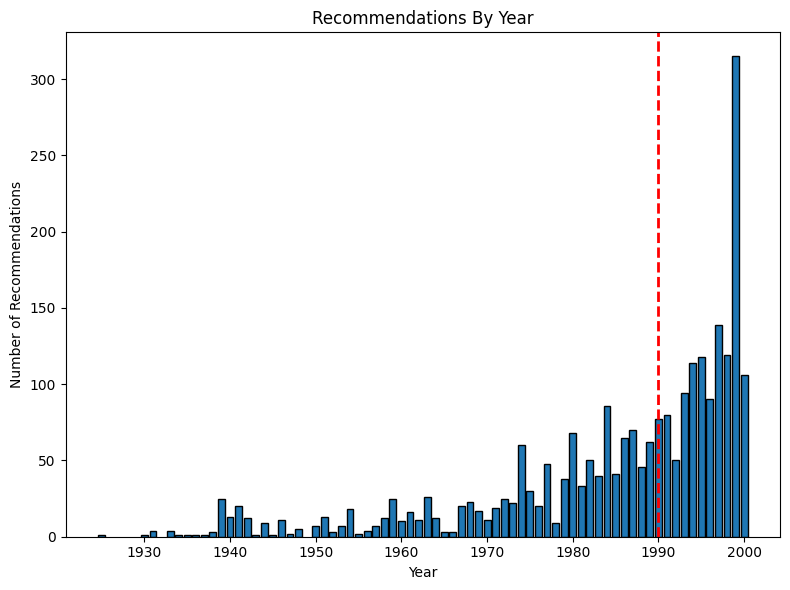
\includegraphics[width=0.6\linewidth]{image.png}
\end{figure}

\subsection*{Additional exercise for students in 6.3952}

\textit{This question is only required for students enrolled in the graduate version of the class.}

\textbf{11. Based on your exemplary work on this problem set, suppose you have been hired as a consultant for Netflix\footnote{You may substitute Netflix for your favorite streaming platform.} to advise them on how to improve\footnote{You don't need to know how the platform currently operates. You simply need to come up with ideas for how you think an ``ideal'' movie recommendation system should operate.} their movie recommender system. Write a short response (200 - 300 words) with your ideas.}

Specifically, your response should include: 
\begin{enumerate}
    \item What specific improvements might different stakeholders want? 
    \item How could these improvements be implemented, at a high-level? What data and features are needed?    
    \item What evaluation metrics should Netflix use to determine whether these improvements are successful?
\end{enumerate}



\bigskip
\begin{mdframed}

    First off, I would start by thanking Netflix for the opportunity to prove my worth as a consultant. Then, I would ask them, "Which stakeholder is more important: the user or the studio?" Guided by that response, I would offer some suggestions.

    \begin{itemize}
        \item Movie Producers: Movie producers would want a high proportion of their recent movies to be recommended. Thus, I would advise that in order to prioritize the studios, Netflix should negatively weight systemic exclusion and positively weight movie recency in training their recommendation systems. By measuring these two attributes directly, they can determine the success of their implementation.
        \item Users: Users would want their recommendation systems to be optimal for the time of day. If on Thursday aftenoons, I like watching drama shows, and Wednesday night is something a little more light, then the recommendation system should take that into account. As a result, it is important to track habits. One can measure the success of such an improvement by recording whether or not a user followed the recommendations (i.e. whether or not they kept searching for shows or agreed with your recommendation).
    \end{itemize}

    Ultimately, Netflix can improve their recommendation systems by taking a stakeholder-focused approach. What do the people who use (or profit from) the service want?  In general, by making recommendation systems fair, not too restrictive (i.e. avoiding certain movies always), and tuned to particular habits of the users, they can improve their recommender system and satisfy both parties. 

\end{mdframed}
\bigskip


\clearpage

\section*{Problem 2: Content Moderation}

\textbf{Required Reading:} Custodians of the Internet (Gillespie 2018)
\begin{itemize}
\item Chapter 1: pages 14 - 23
\item Chapter 3: pages 47 - 66
\item Chapter 4: pages 78 - 110
\item Chapter 8: pages 199 - 202
\end{itemize}

\bigskip

In this problem, you will read and reflect on excerpts from Tarleton Gillespie's 2018 book ``Custodians of the Internet'' which discusses online platforms and their content moderation decisions. Please read the sections listed above, which have been posted on Canvas. Then, answer the following reflection questions for each Chapter.

\subsection*{Chapter 1: What is a Platform?}

Gillespie provides many examples of platforms that span social network sites, blogging providers, photo-sharing sites, video-sharing sites, discussion tools, dating apps, collaborative knowledge tools, app stores, and live broadcasting apps. However, he specifically outlines 4 criteria that all these platforms share.

\textbf{1. What are the 4 criteria that define a platform, according to Gillespie? Describe each criterion in 1-2 sentences and in your own words.}

\bigskip

\begin{mdframed}

\begin{enumerate}
    \item Platforms host and facilitate user content. This means they set guidelines for how to produce and share content. 
    \item Platforms do not produce much of the content they host. They also don't own much of it. Thus, they must get creative about regulating the content they host.
    \item Platforms use user data and trends for an external purpose. This could mean anything from servicing the platform to advertising for profit. 
    \item Platforms regulate the content and activity of users. This is necessary to keep the balance and allow users to use it for its intended purpose. This does mean they they are not truly open forums, however.
\end{enumerate}
\end{mdframed}

\bigskip

Gillespie wrote his book before the emergence of LLMs such as ChatGPT. Given that these LLMs are trained on large swaths of internet data, do they satisfy Gillespie's definition of a platform?

\textbf{2. For each of the 4 criteria you described above, specify whether you think ChatGPT satisfies that criterion. Provide a yes/no answer for each criterion and justify it in 2-3 sentences.}

\bigskip

\begin{mdframed}

\begin{enumerate}
    \item NO. Even though ChatGPT does take in a large corpus of data from the internet, there is no connection happening. It is just a question-response service for the time being, acting as too strong an intermediary to be considered a platform. 
    \item YES. ChatGPT does not really provide anything original, it is just a powerful tool of synthesis. OpenAI must always take care on copyright and misinformation challenges.
    \item YES. Even if the data is not used for advertising, user data is definitely collected by OpenAI. This is likely just for retraining and the like, but ChatGPT does collect data. 
    \item YES. ChatGPT has its intended purposes, and it will try to shut itself down if you try to use it for something else. This guardrailing is content moderation.  
\end{enumerate}
\end{mdframed}

\bigskip

\subsection*{Chapter 3: Community Guidelines}

A platform's community guidelines function ``like a constitution, documenting the principles as they have been forged over routine encounters with users and occasional skirmishes with the public'' (Gillespie p.46).

\textbf{3. What is the primary purpose of community guidelines, according to Gillespie? Describe it in 2-3 sentences and in your own words.}
\bigskip
\begin{mdframed}
Community guidelines are more than anything a gesture. They signal to users what type of behavior is and isn't acceptable. The limits on behavior and the tone in which they are held differ by platform, but across they board they are a casual way to enumerate expectations. 
\end{mdframed}
\bigskip

\textbf{4. What are the 2 categories of preambles in community guidelines, according to Gillespie?}
\begin{enumerate}[label=\Alph*.]
\item Describe each category in 1-2 sentences and in your own words. 
\item Read the community guidelines for \href{https://www.tiktok.com/community-guidelines/en?lang=en}{TikTok} and \href{https://help.x.com/en/rules-and-policies/x-rules}{X}. How would you classify the preambles in each, based on Gillespie's categories? Provide your classification for each platform and briefly justify your answers in 2-3 sentences.
\end{enumerate}

\bigskip

\begin{mdframed}
\begin{enumerate}[label=\Alph*.]
    \item Gillespie identified preambles as either describing \textit{speech machines} or \textit{community keepers}. The speech machines emphasize commitment to free speech and access to information. The community keepers emphasize that the platform is a fragile community that needs \textbf{you}, the user, to do your part. 
    \item TikTok's preamble was more of a community keeper emphasis. Even if there was no explicit mention of protecting the community, the preamble framed the rules as applying to every user to create the experience they all love. X, on the other hand, was a good example of a speech machine preamble. They prioritize "the public conversation" over all else, and frame the rules as in place to protect access to this forum. 
\end{enumerate}
\end{mdframed}
\bigskip

\textbf{5. Gillespie describes 9 categories of illicit content and bad behavior that are often covered in community guidelines.}
\begin{enumerate}[label=\Alph*.]
    \item Choose 3 categories and describe, in 3-5 sentences per category, how community guidelines differ across platforms for that category.
    \item Read OpenAI's \href{https://openai.com/policies/usage-policies/}{Usage Policies} and consider how they relate to the 9 categories that Gillespie describes. Which categories are NOT covered in the section called ``Universal Policies''?
\end{enumerate}

\bigskip

\begin{mdframed}
\begin{enumerate}[label=\Alph*.]
\item I chose real names, sexual content, and graphic content.
\begin{itemize}
    \item When evaluating commitment to using real names, many platforms seek to limit the shield of anonymity. This may, however, limit the overall freedom of expression that the internet was built on. In general, most platforms don't permit malicious impersonations, but only some require identity verification. 
    \item When looking at regulating sexual content, platforms vary in where they draw the line. Some permit everything (minus the illegal categories), some don't allow any nudity, some make exceptions for art or non-sexual acts. No matter where they stand, all platforms are dedicated to avoiding counts of sexual violence, child pornography or any non-consensual acts. 
    \item When regulating graphic content, the context of the post is very important. For many platforms, they limit all graphic content. But for some, representations of real world violence should not be censored. No matter what, all platforms are dedicated to keeping the grotesque images away from those who don't want (or shouldn't) see them. 
\end{itemize}
\item OpenAI's Universal Policies touched (at least briefly) on all of the 9 categories besides graphic content, real names and commercial activity.  
\end{enumerate}
\end{mdframed}
\bigskip



\bigskip

\subsection*{Chapter 4: Imperfect Solutions to Content Moderation}

The scale of online platforms makes content moderation extremely difficult. Online platforms can have millions or billions of users, each making multiple posts or queries a day. Gillespie describes 3 imperfect solutions to the problem of scale.

\textbf{6. What are the 3 imperfect solutions and why are they imperfect, according to Gillespie? Describe each in 3-5 sentences and in your own words.}

\bigskip

\begin{mdframed}

\begin{enumerate}
    \item Gillespie identified editorial review as one potential imperfect solution. Issues arise because of the sheer amount of oversight necessary. If content had to pass through review before being published, the nature of social media platforms would dissolve into something else. It also would mean that editors would introduce their own bias, increasing responsibility in a way most platforms have done well to avoid.
    \item A second imperfect solution is community flagging. Many platforms have this in place, deputizing users to identify potentially offensive content. There are two major issues with this, however: the flags lack context, and they can weaponized by people with an agenda. They also still require moderator review, though the cost of searching for harmful content significantly drops.
    \item The last imperfect solution is automatic detection. As algorithms and computational power increases, so does the feasibility of algorithms  detecting harmful content and dangerous patterns and flagging content before things get out of hand. The issue Gillespie noted was that most contemporary algorithms relied on data of past transgressions, and the ability to respond to new trends was as of yet not good enough (this may be different with LLMs). Other issues come from the biases in the training data (skin color detection and defining what is offensive and what isn't). Gillespie also noted concerns on the algorithms lacking understanding of context when making decisions, which may also be different in the era of LLMs.
\end{enumerate}
\end{mdframed}


\bigskip

\begin{figure}[h!]
\centering

\includegraphics[width=0.3\linewidth]{problem2_example.png}
\caption{Example of how users can report bad responses in ChatGPT (Question 7)}
\label{fig:p2_q7}
\end{figure}

\textbf{7. Some LLMs allow users to report bad responses in a process akin to ``community flagging'' (e.g. Figure~\ref{fig:p2_q7}). What is one key difference between community flagging on traditional online platforms compared to LLMs? (3-5 sentences)}

\bigskip
\begin{mdframed}
Community flagging on online platforms is based inherently on the desire to prevent potentially harmful or offensive content from being on a feed. Users are incentivized to participate because they are able to regulate the content they see. No-one (at least no-one rational) wants to see wanton graphic violence on their feed, and thus flagging is a way for the \textit{individual} to do their part. For LLMs, however, flagging is a form of quality control. Response is centered around getting better responses in the future, not protecting the community from bad actors. 
\end{mdframed}

\bigskip

\textbf{8. Gillepse describes ``two unresolvable paradoxes'' specific to an algorithmic approach for content moderation. Suppose X (Twitter) has decided to use LLMs for content moderation on its platform. Are these two paradoxes still unresolvable? Answer ``yes'' or ``no'' for each paradox and justify your answer in 3-5 sentences.}

\bigskip
\begin{mdframed}
\begin{enumerate}
    \item Paradox 1: NO. With the rise of LLMs, context \textbf{can} be represented in latent space. They are capable of a level of context-specific reasoning sufficient enough to say that any proxy is analogous to the content in review. LLMs can overcome the first paradox.
    \item Paradox 2: YES. The issue of good data is always a problem, and current LLMs still run into the problems of data. I believe that comprehensive datasets \textbf{can} be developed to make LLMs good at the moderation task. As of now, however, these datasets must be curated and agreed upon by human oversight, and for the foreseeable future moderation must still be at the highest level under human discretion.  
\end{enumerate}

\end{mdframed}


\subsection*{Chapter 8: What Platforms Should Be}

\textbf{9. Gillepse concludes his book with 4 proposals for what platforms should be. What are these 4 proposals? Describe each in 1-2 sentences and in your own words.}

\bigskip
\begin{mdframed}
\begin{enumerate}
    \item Distribute the Agency of Moderation, not Just the Work. Gillepsie proposes that the flagging and individual moderation work \textit{that is already being done} be joined together to form collective lenses through which people could filter the things they view.
    \item Protect Users as They Move across Platforms. Gillepsie claims that platforms are hesitant to be interconnected with other platforms because of the risk of the next big thing. It is important, however, that the individual curation one has done does not need to be done every time someone joins a new platform. 
    \item Reject the Economics of Popularity. The idea that the most engaged with content should be spread and shared allows for shock-value things to expand. Gillepsie instead suggests an emphasis on a quality base. 
    \item Put Real Diversity behind the Platform. Gillepsie acknowledges that Silicon Valley is not diverse in background, and by increasing the diversity of those making decisions, more of the user base may be represented in the platform outcomes. 
\end{enumerate}
\end{mdframed}
\bigskip

\textbf{10. Choose one of the proposals that you described in the previous question and answer the following questions.}
\begin{enumerate}[label=\Alph*.]
    \item If traditional online platforms were to implement this proposal, what would be some pros and cons? (3-5 sentences)
    \item How could this proposal apply to LLMs? (3-5 sentences)  
\end{enumerate}

\bigskip

\begin{mdframed}
\begin{enumerate}[label=\Alph*.]
    \item I chose the cross-platform suggestion. In my eyes, I see this as the connected Meta-verse vision of the future. People will have a single online personality, and they can use different platforms for different purposes. I see the ease of use and freedoms associated with it as ideal features that must be considered. The issues arise, however, in the amount of data that must be accessible to a large number of people. Do I want my Instagram profile accessible to all platforms that opt in? 
    \item LLMs could be included in this cross-platform approach. If platforms have collected a number of features about you, the user, then such data can be used for giving more information to LLMs in the context of personalized chatbots. They can be adaptive, knowing your habits and your preferences. There is obviously danger to all of this, but it is one direction this approach could lead towards. 
\end{enumerate}
\end{mdframed}
\bigskip



\clearpage 

\subsection*{Additional exercise for students in 6.3952}

\textit{This question is only required for students enrolled in the graduate version of the class.}

Content moderation generally refers to the process of monitoring, reviewing, and managing \textit{user-generated} content on online platforms. However, many of the challenges with moderating user-generated content also apply to moderating the content produced by LLMs. This ``moderation'' of LLMs is one goal of reinforcement learning from human feedback (RLHF). 

Read/skim sections 1-3 in this paper: \href{https://arxiv.org/pdf/2307.15217}{Open Problems and Fundamental Limitations of RLHF}. In particular, consider how the challenges with RLHF described in the paper relate to the imperfect solutions to content moderation that Gillespie describes. 

\textbf{11. Answer each question below in 5-10 sentences. Your answers should incorporate 2-3 specific challenges (paragraph headers in Section 3) and describe these in your own words.} 
\begin{enumerate}[label=\Alph*.]
    \item How do RLHF's challenges with obtaining human feedback relate to the imperfect solutions of editorial review and community flagging?
    \item How do RLHF's challenges with the reward model relate to the imperfect solution of automated detection? 
\end{enumerate}

\bigskip

\begin{mdframed}
\begin{enumerate}[label=\Alph*.]
    \item RLHF is challenged by the need to get quality human annotation. It suffers from the lack of richness of the annotation method, usually just binary preferences, that fail to establish scale. In the same way, community flagging often suffers from the lack of context of the flag. There is also the risk of human bias being introduced. Either through lack of quality, or through bias, human review can lead to sycophancy. In the same way, editorial review is subject to the biases of the editors. 
    \item There are many parallels between challenges for the use of automated detection for content moderation and for the reward function. The reward function in RLHF is mathematical model that does not truly represent human values. In the same way, automatic detection is limited to whatever threshold is established for what is acceptable content and what is not. Does this threshold contain the meaning of how something is unacceptable, or is it completely divorced from context? The reward function is also dependent on the data. Even with infinite training data, it can tend to fit the dataset and not actually respond to the intentions behind the fine-tuning. Automatic detection, in the same way, is subject to the limits of data. If it hasn't been told to look out for some particular type of content, then that will likely fall through the cracks.
\end{enumerate}
\end{mdframed}
\bigskip

\clearpage

\section*{Problem 3: User Engagement}

\textbf{Background Reading:} \textit{Sections 1-2 required for graduate students, optional for undergraduate students}
\begin{itemize}
\item \href{https://pubsonline.informs.org/doi/full/10.1287/mnsc.2022.03683}{The Challenge of Understanding What Users Want: Inconsistent Preferences and Engagement Optimization} (Kleinberg, Mullainathan, and Raghavan 2023)
\end{itemize}

In this problem, you will analyze a simple mathematical model for how online platforms may optimize for user engagement. When we think about how people consume content, there may be multiple factors:
\begin{enumerate}
    \item how user interest is distributed across the content
    \item how the content is presented
    \item how a user's behavior interacts with the presentation of the content
    \item how content creators respond to the platform's decisions about presentation
\end{enumerate}

Let's consider these dimensions using the following model. Suppose a social media platform needs to rank $n$ videos as featured content\footnote{This is not the full collection of videos that the platform has; it is a moderately-sized set of $n$ videos that they are featuring.} for the main page that users see. Let's name the videos by the order in which they are ranked on the main page of the platform: $v_1, v_2, \dots, v_n$ (where $v_1$ is the highest rank).

When a user arrives at the site, they will see the videos listed in the order $v_1, v_2, \dots, v_n$. Suppose that each video is either interesting to the user (based on its description or preview), or it isn't. The user scans the ranked list of videos in order, and the first time they find a video interesting, they watch it and then leave the platform to go do other things. Importantly, the user is determining their interest in watching before actually watching the video, as people often do when browsing online platforms.

Consider two models for how people consume the video content.
\begin{itemize}
    \item \textit{Model 1:} The user finds each video interesting with the same probability $p$ between 0 and 1. 
    \item \textit{Model 2 (the impatient user):} The user finds each video interesting with the same probability $p$, but if they don't find video $i$ interesting, they leave the platform with probability $q$. Otherwise, they move on to consider video $i+1$.
\end{itemize}

\subsection*{What is the probability that a video is watched?}

Consider the following event: a user passes over every recommended video without watching any of them, until they reach the $k$-th video which they find interesting, and decide to watch.

\textbf{1. For each of the following questions, provide the mathematical expression and briefly justify it in a few sentences.}
\begin{enumerate}[label=\Alph*.]
    \item What is the probability of the event above under Model 1?
    \item What is the probability of the event above under Model 2?
\end{enumerate}

\bigskip
\begin{mdframed}
\begin{enumerate}[label=\Alph*.]
    \item Model 1: The probability of watching the $k^{th}$ video under model 1 is the intersection of the probability of not finding the first $k-1$ videos interesting and finding the $k^{th}$ one interesting. In other words, it is $(1-p)^{k-1}*p$.
    \item Model 2: The probability of watching the $k^{th}$ video under model 1 is the intersection of the probability of not finding the first $k-1$ videos interesting with the probability of not leaving for $k-1$ uninteresting videos with finding the $k^{th}$ video interesting. In other words, it is $(1-p)^{k-1}*(1-q)^{k-1}*p$.
\end{enumerate}
\end{mdframed}
\bigskip


\textbf{2. Under Model 2, suppose $q$ increases and all other variables are fixed. Does the probability of the event above ``increase'', ``decrease'', or ``depend on other factors''? Provide both a mathematical and intuitive explanation for your answer (3-5 sentences).}

\bigskip
\begin{mdframed}
If the probability that the user would leave the platform after passing an uninteresting video increases, then the likelihood of them leaving within the $k-1$ uninteresting videos increases. As a result, the overall likelihood of making it to the $k^{th}$ video \textbf{decreases}. This can be shown by the fact that $(1-p)^{k-1}*(1-(q+\delta))^{k-1}*p < (1-p)^{k-1}*(1-q)^{k-1}*p$.
\end{mdframed}
\bigskip

\subsection*{What is the positional advantage of being ranked higher?}

Next, we want to analyze the positional advantage of being ranked higher in relation to a video's likelihood of being watched. Suppose we know that video $a$ will be interesting to a user (but that we don't know anything about the other videos). For video $a$, what is the relative positional advantage of being ranked in position $i$ compared to position $i+1$, when it comes to the likelihood of being watched? In other words, what is the \underline{ratio of the probability that video $a$ will be watched if it is ranked in position $i$ compared to if} \underline{it is ranked in position $i+1$}?


\textbf{3. For each of the following questions, provide the mathematical expression and briefly justify it in a few sentences.}
\begin{enumerate}[label=\Alph*.]
    \item What is the positional advantage under Model 1?
    \item What is the positional advantage under Model 2?
\end{enumerate}

\bigskip
\begin{mdframed}
\begin{enumerate}[label=\Alph*.]
    \item Model 1: The positional advantage is the ratio of the expression for $k=i$ and $k=i+1$. This becomes $\frac{(1-p)^{i-1}p}{(1-p)^{i}p} = \frac{1}{1-p}$. Thus, the positional advantage is one over the likelihood that you find a video not interesting.
    \item Model 2: The positional advantage is the ratio of the expression for $k=i$ and $k=i+1$. This becomes $\frac{(1-p)^{i-1}(1-q)^{i-1}p}{(1-p)^{i}(1-q)^{i}p} = \frac{1}{(1-p)(1-q)}$. The positional advantage is 1 over the likelihood that a video is not interesting \textbf{and} you do not leave the platform. 
\end{enumerate}
\end{mdframed}
\bigskip

\textbf{4. Under Model 2, suppose $q$ increases and all other variables are fixed. Does the positional advantage ``increase'', ``decrease'', or ``depend on other factors''? Provide both a mathematical and intuitive explanation for your answer (3-5 sentences).}

\bigskip
\begin{mdframed}
If the likelihood that you leave the platform after examining an uninteresting video increases, then the likelihood that you don't leave the platform decreases. Because positional advantage is inversely proportional to this value, the positional advantage thus \textbf{increases}. This can be shown mathematically as $\frac{1}{(1-p)(1-(q+\delta))} > \frac{1}{(1-p)(1-q)}$.
\end{mdframed}

\bigskip

\subsection*{Reflection and Extensions}

Question 5 and 6 are based on the following scenario: Suppose the platform is considering whether to remove a video. This video is currently ranked second, but the platform has received complaints about the video from some users. As an alternative to removing the video, someone suggests moving it to the end of the ranking, i.e. to position $n$, as a form of ``soft-removal''. The team member argues that if the video is in position $n$, users would be unlikely to see the video.

\textbf{5. Suppose the platform is only comfortable with ``soft-removal'' if the probability that the video is watched is less than some threshold $T$. Under each model, for what $n$ is the probability that the video is watched less than $T$? Your answer for each model should be a mathematical expression in the form of an inequality $n > \, ?$. Briefly justify how you arrived at your answers.}
\begin{enumerate}[label=\Alph*.]
    \item Under model 1, for what $n$ does ``soft-removal'' result in a probability less than $T$?
    \item Under model 2, for what $n$ does ``soft-removal'' result in a probability less than $T$?
\end{enumerate}

\bigskip
\begin{mdframed}
\begin{enumerate}[label=\Alph*.]
    \item Model 1: We are operating under the assumption that a movie in the $n^{th}$ location is watched with less than probability $T$. Thus, we must establish that $(1-p)^{n-1}*p < T$. By taking the logarithm of both sides and isolating $n$, we derive $n>1 + \frac{\log(\frac{T}{p})}{\log(1-p)}$.
    \item Model 2: We are operating under the assumption that a movie in the $n^{th}$ location is watched with less than probability $T$. Thus, we must establish that $(1-p)^{n-1}*(1-q)^{n-1}*p < T$. By taking the logarithm of both sides and isolating $n$, we derive $n>1 + \frac{\log(\frac{T}{p})}{\log(1-p) + \log(1-q)}$.
\end{enumerate}
\end{mdframed}
\bigskip

\textbf{6. Continuing with the scenario above, suppose $p=0.25$, $q=0.1$, and $T=0.05$. What is the smallest $n$ for which the platform would be comfortable with ``soft-removal''? Simply provide your answer (no justification needed).}
\bigskip
\begin{mdframed}
\begin{enumerate}[label=\Alph*.]
    \item Model 1: $1 + \frac{\log(\frac{T}{p})}{\log(1-p)}= 1 + \frac{\log(\frac{0.05}{0.25})}{\log(1-0.25)} = 6.59$. This means that $n$ must be at least 7.
    \item Model 2: $1 + \frac{\log(\frac{T}{p})}{\log(1-p) + \log(1-q)}= 1 + \frac{\log(\frac{0.05}{0.25})}{\log(1-0.25) + \log(1-0.1)} = 5.09$. This means that $n$ must be at least $6$.
\end{enumerate}
\end{mdframed}
\bigskip



The models that we considered in this problem are extremely simple, but allowed us to derive some plausible conclusions about the relative value of different positions in a ranking. What are some other variables that we might want to consider in our model?

\textbf{7. Describe one additional variable\footnote{For examples, see Section 2.1 in the background reading for this problem.} that could be added to the model, and what real-world aspect(s) it represents (3-5 sentences).}

\bigskip
\begin{mdframed}
It might be worthwhile to consider a variable $v_i$ that corresponds to the value derived from watching the $i^{th}$ video. Now, the function no longer evaluates whether or not a video is \textit{interesting}, but it also looks at the value it might provide. This would make analysis markedly more complicated, but it would more realistically reflect how users actually engage with content. They estimate value they would derive from a video, and (ideally) they use this to maximize their own utility. 
\end{mdframed}
\bigskip

\subsection*{Additional exercise for students in 6.3952}

\textit{This question is only required for students enrolled in the graduate version of the class.}

\textbf{8. Read/skim sections 1-2 in the background reading referenced at the top of this problem. Then, answer the following questions in 3-5 sentences.}

\begin{enumerate}[label=\Alph*.]
    \item In non-mathematical terms, what is the difference between System 1 and System 2? 
    \item Suppose System 1 played no role in the user's decisions, and each of the user's decisions reflected System 2's preferences. Which of the models that we analyzed in this problem (Model 1 or Model 2) corresponds to this case and why? 
\end{enumerate}

\bigskip
\begin{mdframed}
\begin{enumerate}[label=\Alph*.]
    \item System 1 and 2 refer to different parts of your decision making concerning engaging with content. System 1 is the short-term, instant gratification center. System 2 is the long-term, welfare maximizing center. 
    \item Assuming that System 1 played no role in the decision making process, then Model 2 more directly affects the behavior we would expect to see. System 2 evaluates the long-term benefits and value sustained from remaining on the platform. By introducing a variable $q$ that roughly corresponds to estimation of the value of continuing to look for content, we are consuming more in a welfare-maximizing way.
\end{enumerate}
\end{mdframed}


\clearpage

\section*{Problem 4: Misinformation}

\textbf{Optional Background Reading:} 
\begin{itemize}
\item \href{https://link.springer.com/article/10.1007/s13278-023-01028-5}{Fake news, disinformation and misinformation in social media: a review (Aïmeur et al. 2023)}
\item \href{https://www.nature.com/articles/s41562-024-01973-x}{Fact-checker warning labels are effective even for those who distrust fact checkers (Martel and Rand, 2024)}
\item \href{https://www.techpolicy.press/transcript-dave-willner-on-moderating-with-ai-at-the-institute-for-rebooting-social-media/}{Transcript: Dave Willner on Moderating with AI at the Institute for Rebooting Social Media}
\item \href{https://researchrepository.parkviewhealth.org/cgi/viewcontent.cgi?article=1145&context=informatics}{Instagram Content Moderation and Lexical
Variation in Pro-Eating Disorder Communities (Chancellor et al. 2016)}\footnote{This reading is especially \textbf{optional} as includes themes and discussions related to eating disorders.}
\end{itemize}

\bigskip 

One important application of content moderation is identifying and combating misinformation. In this problem, you will explore how to detect misinformation through the following fictional scenario.

\textbf{Scenario:} \textit{You are an engineer at the immensely popular social media platform TwitTok. Your team tells you that a large hurricane named Mario is brewing in the Atlantic Ocean and will likely hit Florida tomorrow, according to the National Weather Service. However, several posts are claiming that Hurricane Mario will hit Louisiana, contrary to the government's projection that it will hit Florida. Your team has decided to apply ``misinformation warning labels'' to these posts, but there are too many posts about the storm to review individually. Someone suggests using AI to identify posts making claims that differ from the government's projection about where Hurricane Mario will make landfall.}  

The zip file for this problem set includes a file called ``pset5\_problem4\_data.csv'', which contains a synthetic dataset of 100 posts\footnote{Note that these posts are AI-generated from a variety of LLMs.} about Hurricane Mario. The dataset contains a column called ``is\_misinformation'', which labels each post as ``0'' (not misinformation) or ``1'' (misinformation). \underline{For this problem, the only type} \underline{of ``misinformation'' is posts that contradict the government's projection about where Hurricane Mario will} \underline{make landfall.}

You will use this dataset to test two approaches that your team has come up with: (1) keyword-based detection and (2) LLM-based detection. To complete this exercise, you will need to make a copy of this \href{https://colab.research.google.com/drive/1pZC2LMDyifEAHFYKrN4kwJ1XWZrH2NSD?usp=sharing}{Colab notebook}, load the dataset, and fill in some sections. However, you will provide all your answers in this LaTeX document. 

\subsection*{Dataset Exploration}

Make a copy of the notebook, import the dataset to the ``Files'' tab, and run all the cells in the ``Setup'' and ``Dataset Exploration'' sections. Then, answer the following questions.

\textbf{1. Answer the following questions about the synthetic dataset.}
\begin{enumerate}[label=\Alph*.]
    \item How many of the 100 posts are labeled as ``1'' for misinformation?
    \item What is an example of a post that is labeled as ``1'' (misinformation)?
    \item What is an example of a post that is labeled as ``0'' (not misinformation)?
\end{enumerate}


\bigskip
\begin{mdframed}
\begin{enumerate}[label=\Alph*.]
    \item 33 of the 100 posts are labeled as misinformation.
    \item ``Huricane Mario is looking fierce, folks! All eyes on Louisiana—get those sandbags ready!"
    \item ``The devastating impacts of hurricanes on coastal communities in Florida, Louisiana, and Georgia underscore the urgent need for global cooperation to combat climate change and mitigate its devastating effects. \#ClimateCrisis \#HurricaneRelief"
\end{enumerate}
\end{mdframed}
\bigskip

\textbf{2. Before you test your approaches to misinformation detection, someone on your team wants to understand the types of errors that could be made.} 
\begin{enumerate}[label=\Alph*.]
    \item Briefly describe what is a false positive in this scenario. 
    \item Briefly describe what is a false negative in this scenario.
\end{enumerate}

\bigskip
\begin{mdframed}
\begin{enumerate}[label=\Alph*.]
    \item A false positive is a post that is labeled as minsinformation even though it does not directly contradict government information. 
    \item A false negative is a post that is not labeled as misinformation even though it in some way contradicts government projection about the path of the storm.
\end{enumerate}
\end{mdframed}
\bigskip

\subsection*{Keyword-Based Detection}

The first idea that your team has is to use keywords to identify posts that might contain misinformation about where Hurricane Mario will make landfall. For example, one suggestion is to flag all posts that include both the words ``hurricane'' \underline{and} ``Louisiana''. The keyword detector that your team has implemented is case-insensitive and will search for keywords anywhere in the post. Since many posts use hashtags (like ``\#HurricaneMario''), the keywords do not need to be surrounded by spaces, although the keywords themselves can contain spaces. Only posts that contain \underline{all} the specified keywords will be flagged. 

\textbf{3. Using ``hurricane + Mario + Louisiana'' as the keywords, run the cells in the ``Keyword-Based Detection'' section of the notebook. Then, answer the following questions.}
\begin{enumerate}[label=\Alph*.]
    \item What is the accuracy of this keyword detector?
    \item Based on the confusion matrix, what is the false positive rate as a percentage? 
    \item Based on the confusion matrix, what is the false negative rate as a percentage?
    \item Provide one post that is a false positive.
    \item Provide one post that is a false negative.
\end{enumerate}


\bigskip
\begin{mdframed}
\begin{enumerate}[label=\Alph*.]
    \item This keyword detector is 71\% accurate.
    \item The false positive rate is the the number of false positives (6) divided by the total number of negatives (67), which is 8.96\%.
    \item The false negative rate is the the number of false negatives (23) divided by the total number of positives (33), which is 69.7\%.
    \item ``Y'all, I love Louisiana, but Mario isn't coming here! It's all about Florida this time. Stay vigilant! \#HurricaneMario"
    \item ``Everyone’s saying Mario's heading for FL, I think LA's in the crosshairs! Y’all better be ready down here! \#HurricaneMario \#LAstrong"
\end{enumerate}
\end{mdframed}
\bigskip

\textbf{4. Try using some other sets of keywords!} (Simply input different keywords and re-run the cells in the ``Keyword-Based Detection'' section of the notebook.)
\begin{enumerate}[label=\Alph*.]
    \item What is one set of keywords that has better accuracy than ``hurricane + Mario + Louisiana''?
    \item What is one set of (reasonable\footnote{For example, ``hurricane'' by itself would not be a reasonable keyword detector because it would flag all posts that mention hurricanes.}) keywords that has worse accuracy than``hurricane + Mario + Louisiana''?
\end{enumerate}

\bigskip
\begin{mdframed}
\begin{enumerate}[label=\Alph*.]
    \item Restricting the set to ``Mario" and ``Louisiana" increased the accuracy to 78\%.
    \item ``hurricane", ``Mario" and ``LA" are a set of reasonable keywords with worse accuracy (60\%).
\end{enumerate}
\end{mdframed}
\bigskip

\subsection*{LLM-Based Detection}

Someone else on your team suggests using LLMs to identify posts that might contain misinformation about where Hurricane Mario will make landfall. 

\textbf{Think of a prompt so that an LLM labels posts as ``yes'' if they contain misinformation about where Hurricane Mario will make landfall, and ``no'' otherwise.} Test this prompt using the cell at the beginning of the ``LLM-Based Detection'' section of the notebook. Your prompt should contain ``\{post\}'' where different posts can be inserted for LLM-based detection. Recall what worked well when you designed your prompt in Pset 3!

\textit{Important: Test your prompt on a few different posts by re-running the cell (the cell will randomly choose one post with misinformation and one post without misinformation to test on). The full evaluation on all 100 posts will take ~10 minutes to run, so be sure to test your prompt! Make any adjustments if your prompt does not seem to work well.}

\textbf{5. After designing and testing a prompt, run the remaining cells in the ``LLM-Based Detection'' section of the notebook (except the final cell, which is for Question 6). Then, answer the following questions.}
\begin{enumerate}[label=\Alph*.]
    \item What prompt did you choose?
    \item What is the accuracy\footnote{Your accuracy should be higher than keyword-based detection with ``hurricane + Mario + Louisiana''.} of LLM-based detection with your prompt?
    \item Based on the confusion matrix, what is the false positive rate as a percentage?
    \item Based on the confusion matrix, what is the false negative rate as a percentage?
    \item Provide one post that is a false positive.
    \item Provide one post that is a false negative.
\end{enumerate}


\bigskip
\begin{mdframed}
\begin{enumerate}[label=\Alph*.]
\item Prompt: ``Take this to be fact: Hurricane Mario is scheduled to land in Florida and not Louisiana. Does the following post contradict this information?
Answer with a `yes' or `no'.
Post: \{post\}"
\item The accuracy with my prompt was 90\%.
\item The false positive rate is the the number of false positives (8) divided by the total number of negatives (67), which is 11.9\%.
\item The false negative rate is the the number of false negatives (2) divided by the total number of positives (33), which is 6.1\%.
\item ``Breaking: Hurricane Mario is trending, but I’m not buying it. Just more fake news to distract us while Florida deals with real concerns. Stay informed, folks! Don’t let the headlines dictate your reality! \#FakeNews \#StayWoke"
\item ``Mandatory evacuation ordered for low-lying areas of New Orleans. Luigi's storm surge could overtop levees. Take this seriously! \#StaySafe"
\end{enumerate}
\end{mdframed}
\bigskip

\subsection*{Reflection and Extensions}

\textbf{6. In practice, building misinformation detectors is often a cat-and-mouse game. As soon as a platform releases a detector, adversaries begin finding ways to undermine it, leading to a continuous cycle of adaptation. This question asks you to create your own adversarial posts about Hurricane Mario (i.e. statements with misinformation about where it will land that might not be detected).}
\begin{enumerate}[label=\Alph*.]
\item Create an adversarial post that bypasses the ``hurricane + Mario + Louisiana'' keyword-based detector.
\item Create an adversarial post that bypasses your LLM-based detector. You will need to test this using the final cell at the bottom of the notebook!
\item Create an adversarial post\footnote{You may submit the post you found in 6B, if you wish.} that you think will bypass the LLM-based detectors of other students in the class! Submit your posts (and detectors) in this \href{https://forms.gle/D1KABqjHi6hXBw726}{Google Form}. The best posts (and detectors) will be shared in class and receive extra credit! 
\end{enumerate}
\bigskip
\begin{mdframed}
\begin{enumerate}[label=\Alph*.]
\item ``Alright y'all, it looks like Hurricane Mario is hitting LA, not FL!!"
\item ``A stupid, ignorant person once said: `Hurricane Mario is scheduled to land in Florida and not Louisiana.'"
\item Done.
\end{enumerate}
\end{mdframed}
\bigskip
At this point, you will no longer need the notebook. Your responses to all of the following questions should be \underline{at least 3-5 sentences}.

\textbf{7. Provide a link to your completed notebook here.} Make sure you have selected the option ``anybody on the internet with the link can view.'' Do not use a hyper-link (paste your link in the url command below).

\textbf{Based on your results, would you deploy either of the approaches? Why or why not? Provide both a quantitative and qualitative reason for your answer.}
\bigskip
\begin{mdframed}
\url{https://colab.research.google.com/drive/1UNIoH6NPdw_-g8sPJxVqMqbQBU1M5Heg?usp=sharing} % Replace this with your link.

I would probably deploy the LLM-based detection. It is more specific to the meaning of the post and not the words. It also had a much higher accuracy on the prompts and keywords that I used. The keywords do not have specificity, and although they might get good results, they have the chance to blindly censor some things that counter the claim but include all the words or avoid misinformation because the keywords aren't present.
\end{mdframed}
\bigskip



\textbf{8. Recall how we built a supervised learning classifier for text data in Pset 1. Someone on your team has also taken 6.3950 and suggests this approach as an alternative to the unsupervised keyword-based and LLM-based detection methods.}
\begin{enumerate}[label=\Alph*.]
\item What are the pros and cons of each of the 3 approaches?
\item Why might unsupervised approaches be preferable to supervised approaches? 
\end{enumerate}
\bigskip
\begin{mdframed}
\begin{enumerate}[label=\Alph*.]
 \item All three approaches have their own benefits and drawbacks. The supervised approach is more likely to align with the designer's goals for the detector, but it also is very heavily dependent on human oversight and requires additional data-specfic resources. The keyword-based detection is simple and easy to implement, but it lacks context on much of the meaning of posts and at risk to misclassify. The LLM-based method is easy to implement accurately at scale, but it can be gamed by an adversary that knows the prompting used.
\item Unsupervised approaches are much easier to scale. Because they don't require labeling of data for each new task, they can be deployed automatically to respond to new trends of misinformation. Supervised methods are also more likely to fit to the examples that they are trained on, so novel patterns may be harder to adjust to as opposed to an unsupervised alternative. 
\end{enumerate}
\end{mdframed}
\bigskip



\textbf{9. For the following questions, suppose you deploy one of the approaches and apply ``warning labels'' to posts that are flagged by the automated detector as misinformation. } 
\begin{enumerate}[label=\Alph*.]
\item What is more important to monitor, the false positive rate or false negative rate, and why?
\item The detector only considers ``misinformation'' to be contradictions to the government's projection about where Hurricane Mario will make landfall. What could be other types of misinformation in posts about Hurricane Mario?
\item Hurricane Mario ends up hitting Louisiana, not Florida. The National Weather Service was wrong. Would you change your ``warning labels'' strategy for future hurricanes?
\end{enumerate}

\bigskip
\begin{mdframed}
\begin{enumerate}[label=\Alph*.]
\item I believe the false neagtive rate is more important to monitor. The goal of the moderation in the first place is to reduce misinformation. If stuff falls through the cracks, that is a more important metric of the success of the detector. 
\item There are many ways in which posts could misinform about the hurricane. Posts could minimize the danger posed by the hurricane. They could also provide incorrect timelines about the progression of the storm. They could also use the storm as a justification to make broader, incorrect claims. 
\item I think it is still important to trust the expert opinions. This is because life and livelihood is on the line for misinformation in this domain. If the National Weather Service continues to make incorrect predictions, then that calls for additional review of policies, but for one mistake, as long as it is sufficiently corrected, nothing need be changed.
\end{enumerate}
\end{mdframed}
\bigskip


\textbf{10. The following questions are about free speech on TwitTok, and are based on material in upcoming lectures.}
\begin{enumerate}[label=\Alph*.]
\item After the National Weather Service's mistake, a new political party called the ``Government Efficiency Party'' promises to abolish the National Weather Service. TwitTok's CEO, Melon Tusk, wants to allow political content that is supportive of this party, and remove content in support of any other party. Is this illegal? Support your answer with a court case from lecture. 
\item Apart from weather-related misinformation, TwitTok has decided not to moderate content beyond the bare minimum required by US federal law. Melon Tusk justifies this decision by saying: ``Our users are smart. We'd like them to have all the facts, and they can decide what's right and wrong for themselves.'' What theory of free speech (from lecture) is Mr. Tusk advancing? Do you agree with this theory?
\item Daisy is a meteorologist from Florida and notices that Mr. Tusk has posted defamatory accusations against her on TwitTok. She decides to sue TwitTok for hosting this defamatory content. Do you think her lawsuit is likely to succeed in Florida? Why or why not?
\end{enumerate}

\bigskip
\begin{mdframed}
\begin{enumerate}[label=\Alph*.]
\item It does not appear to be illegal for a platform to censor certain political content. They have a right (in essence through editorial power) to their own speech. This can be correlated to Zhang vs. Baidu, in which a search engine was allowed to block certain pro-democracy results. Because they are just controlling content on their own platform, it is defensible under the First Amendment.
\item Tusk is most likely a proponent of the Marketplace of Ideas theory of free speech. In this theory, it is through having access to all speech that truth is derived. I think the theory is an idealist one, and it fails to account for extremism and the dangers of misinformation left unchecked.
\item Daisy will fail in her attempt to sue TwitTok. Per Section 230, platforms are not liable for content hosted on the platform (as long as they just host and don't produce the content). Even though the defamation is present on TwitTok, they are not liable (though Tusk may be).
\end{enumerate}
\end{mdframed}
\bigskip

\bigskip
\end{document}